% Generated by thesis/ch7/exp2/worked.py -- do not edit by hand.
\begin{figure}[tbp]
  \centering
  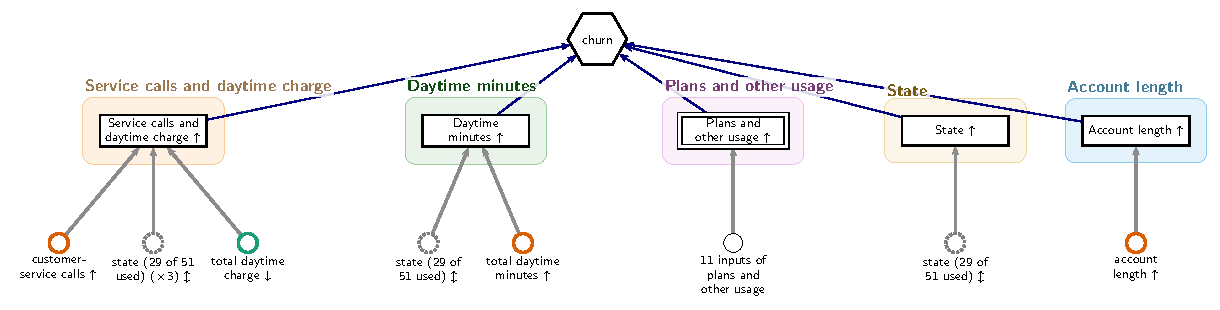
\includegraphics[width=\textwidth,height=0.8\textheight,keepaspectratio]{figures/ch7/used/exp2-worked-net-concept}
  \caption{Churn seed 5 at the level of concepts: each top-level part of the explanation collapsed into one box, the inputs each reads, and the churn score at the top. Arrows on inputs and boxes: the direction of the effect on the final prediction (up raises it, down lowers it, double arrow depends). Edges: blue, a positive weight (raises the score); red, a negative weight; thicker, a larger weight; grey, the inputs a collapsed part reads (no single weight). A grouped input (state) stands for its used levels.}
  \label{fig:exp2-worked-net-concept}
\end{figure}
